\begin{center}
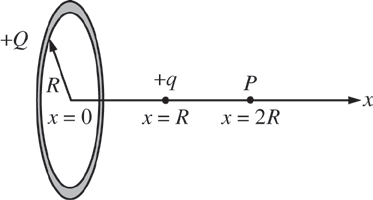
\includegraphics[scale=0.5]{images/img-007-019.png}
\end{center}

% Multiple Choice Question 24
\begin{questions}\setcounter{question}{23}\question
A thin ring of radius $R$ has charge $+Q$ distributed uniformly around the ring. The center of the ring is at the origin of an $x$-axis perpendicular to the plane of the ring, as shown in the figure above. A point charge $+q$ on the $x$-axis at position $x=R$ is released from rest. What is its kinetic energy when it reaches position $P$ at $x=2 R$ on the $x$-axis?

\begin{oneparchoices}
\choice $\dfrac{3}{10} \dfrac{k Q q}{R}$
\choice $\dfrac{1}{2} \dfrac{k Q q}{R}$
\choice $\dfrac{1}{\sqrt{3}} \dfrac{k Q q}{R}$
\choice $\dfrac{k Q q}{R}$
\choice $\dfrac{k Q q}{R}\left(\dfrac{1}{\sqrt{2}}-\dfrac{1}{\sqrt{5}}\right)$
\end{oneparchoices}\end{questions}

